% KSe.tex
% $Author$ $Date$

\section{\KSe}
\label{s-KS}

The \KS\ [henceforth KS] system\rf{ku,siv},
which arises in the description of
stability of flame fronts, reaction-diffusion systems and many other
physical settings\rf{KNSks90}, is one of the simplest nonlinear PDEs that
exhibit spatiotemporally chaotic behavior. In the formulation
adopted here, the time evolution of the `flame front velocity'
$u=u(x,t)$ on a periodic domain $u(x,t) = u(x+L,t)$ is given by
\beq
  u_t = F(u) = -{\textstyle\frac{1}{2}}(u^2)_x-u_{xx}-u_{xxxx}
    \,,\qquad   x \in [-L/2,L/2]
    \,.
\ee{ks}
Here $t \geq 0$ is the time, and $x$ is the spatial coordinate.
The subscripts $x$ and $t$ denote partial derivatives with respect to
$x$ and $t$. In what follows
we shall state results of all calculations either in units of the
`dimensionless system size' $\tildeL$, or the system size $L = 2 \pi
\tildeL$. \refFig{f:ks_largeL} presents a typical `turbulent' evolution
for KS. All numerical results presented in this paper
are for the system size $\tildeL=22/2\pi = 3.5014\ldots$, for which a
structurally stable chaotic attractor is observed (see \reffig{f:ks_L22}).
Spatial periodicity $u(x,t)=u(x+L,t)$
makes it convenient to work in the Fourier space,
\beq
  u(x,t)=\sum_{k=-\infty}^{+\infty} a_k (t) e^{ i k x /\tildeL }
\,,
\ee{eq:ksexp}
with the $1$-dimensional PDE \refeq{ks}
replaced by an infinite set of
ODEs for the complex Fourier coefficients $a_k(t)$:
\beq
\dot{a}_k= \pVeloc_k(a)
     = ( q_k^2 - q_k^4 )\, a_k
    - i \frac{q_k}{2} \sum_{m=-\infty}^{+\infty} a_m a_{k-m}
\,,
\ee{expan}
where $q_k = k/\tildeL$.
Since $u(x,t)$ is real, $a_k=a_{-k}^\ast$, and we can replace the
sum by an $m > 0$ sum.

Due to the hyperviscous damping $u_{xxxx}$, long time solutions of KS
equation are smooth, $a_k$ drop off fast
with $k$, and truncations of \refeq{expan} to $16 \leq N \leq 128$
terms yield accurate solutions for system sizes considered here (see
\refappe{sec:fourierRLD}).  Robustness of the long-time dynamics
of KS as a function of the number of Fourier modes kept in truncations
of \refeq{expan} is, however, a subtle issue.  Adding an extra mode to
a truncation of the system introduces a small perturbation in the
space of dynamical systems.  However, due to the lack of structural
stability both as a function of truncation $N$, and the system size
$L$, a small variation in a system parameter can (and often will)
throw the dynamics into a different asymptotic state.  For example,
asymptotic attractor which appears to be chaotic in a $N$-dimensional
\statesp\ truncation can collapse into an attractive cycle
for $(N\!+\!1)$-dimensions.
Therefore, the selection of parameter $L$ for which a
structurally stable chaotic dynamics exists and can be
studied is rather subtle. We have found that the value of $L
= 22$ studied in \refsect{sec:L22} satisfies these
requirements. In particular, all of the equilibria and
relative equilibria persist and remain unstable when $N$ is
increased from 32 (the value we use in our numerical
investigations) to 64 and 128.  Nearly all of the \rpo s we
have found for this system also exist and remain unstable for
larger values of $N$ as well as smaller values of the
integration step size (see \refappe{sec:lmderRLD} for
details).

%%%%%%%%%%%%%%%%%%%%%%%%%%%%%%%%%%%%%%%%%%%%%%%%%%%%%%%%%%%%%%
\begin{figure}[t]
\begin{center}
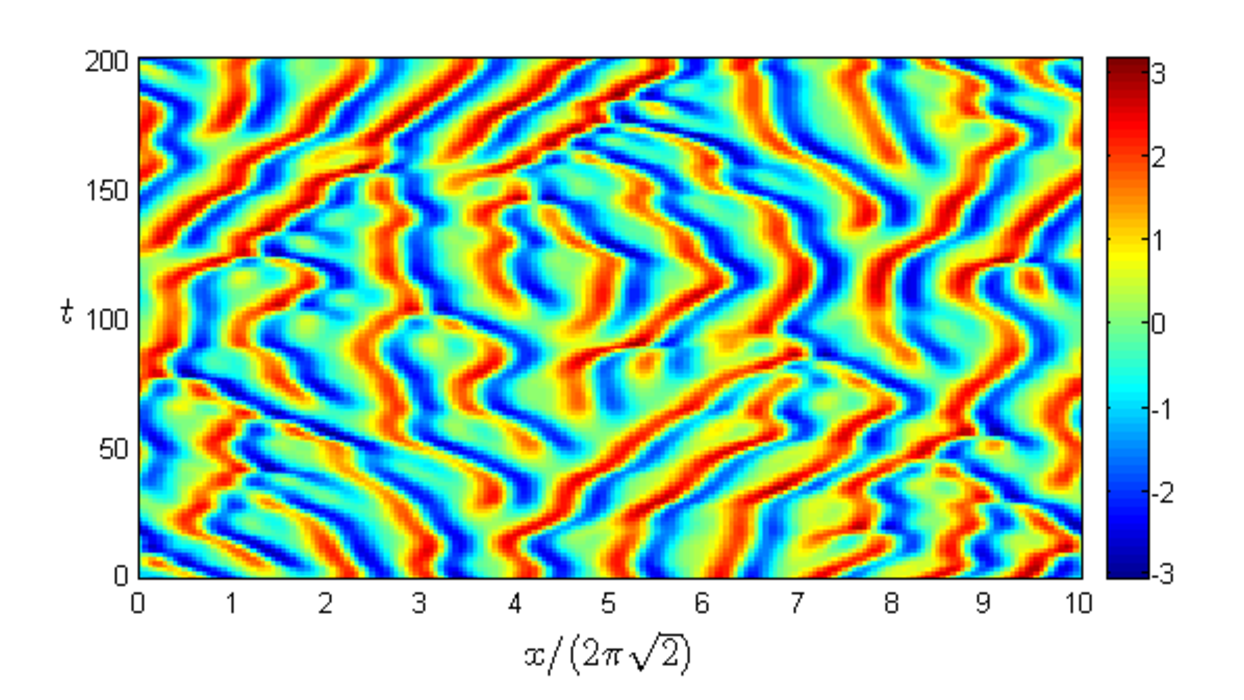
\includegraphics[width=0.9\textwidth]{figs_bmp/ks_largeL_cbar_200.eps} 
\end{center}
\caption{
A typical spatiotemporally chaotic solution of the \KSe, system size
$L=20\pi\sqrt{2}\approx 88.86$.  The $x$ coordinate is scaled
with the most unstable wavelength $2\pi\sqrt{2}$, which is
approximately also the mean wavelength of the turbulent flow.
The color bar indicates the color scheme for $u(x,t)$, used also
for the subsequent figures of this type.
     } \label{f:ks_largeL}
\end{figure}
%%%%%%%%%%%%%%%%%%%%%%%%%%%%%%%%%%%%%%%%%%%%%%%%%%%%%%%%%%%%%%%%%%

\subsection{Symmetries of \KSe}
\label{sec:KSeSymm}

The KS equation is Galilean invariant: if $u(x,t)$ is a solution,
then $u(x -ct,t) -c $, with $c$ an arbitrary constant
speed, is also a solution. Without loss of generality, in our
calculations we shall set the mean velocity of the front to zero,
\beq \int dx \, u = 0 \,. \ee{GalInv}
As $\dot{a_0}=0$ in
\refeq{expan}, $a_0$ is a conserved quantity
fixed to $a_0=0$ by the condition \refeq{GalInv}. $G$, the group of actions $ g \in G $ on a
\statesp\ (reflections, translations, \etc) is a symmetry of the KS
flow \refeq{ks} if $g\,u_t = F(g\,u)$.
The KS equation is time translationally invariant, and space translationally invariant
on a periodic domain under
the 1-parameter group of
$O(2): \{\Shift_{\shift/L},\Refl \}$.
If $u(x,t)$ is a solution, then
$\Shift_{\shift/L}\, u(x,t) = u(x+\shift,t)$
is an equivalent solution for any shift
$-L/2 < \shift \leq L/2$,
as is the
reflection (`parity' or `inversion')
\beq
    \Refl \, u(x) = -u(-x)
\,.
\ee{KSparity}
The translation operator action on the Fourier coefficients \refeq{eq:ksexp},
represented here by a complex valued vector
$a = \{a_k\in\mathbb{C}\,|\,k = 1, 2, \ldots\}$, is given by
\beq
  \Shift_{\shift/L}\, a = \mathbf{g}(\shift) \, a \,,
  \label{eq:shiftFour}
\eeq
where $\mathbf{g}(\shift) = \diag( e^{i q_k\, \shift} )$ is a complex
valued diagonal matrix, which amounts to the $k$-th mode complex plane
rotation by an angle $k\, \shift /\tildeL$.  The reflection acts on
the Fourier coefficients by complex conjugation,
\beq
  \Refl \, a = -a^\ast
\,.
\ee{FModInvSymm}
Reflection generates the dihedral subgroup $D_1 = \{1, \Refl\}$
of $O(2)$.  Let $\bbU$ be the space of
real-valued velocity fields periodic and square integrable
on the interval $\Omega = [-L/2,L/2]$,
\begin{align}
 \bbU  &= \{u \in L^2(\Omega) \; | \; u(x) = u(x+L)\}  \,.
\end{align}
A continuous symmetry maps each state $u \in \bbU$
to a manifold of functions with identical dynamic behavior.
Relation $\Refl^2 = 1$ induces linear decomposition
$u(x) = u^+(x)+ u^-(x)$,
$u^\pm(x)= P^\pm u(x) \in  \bbU^\pm$,
into irreducible subspaces
$
\bbU = \bbU^+
       \oplus \bbU^-
$, where
\beq
    P^+=(1+\Refl)/2
    \,,\qquad
    P^-=(1-\Refl)/2
\,,
\ee{P1P2proj} are the antisymmetric/symmetric projection operators.
Applying $P^+,\,P^-$ on the KS equation \refeq{ks} we have\rf{KNSks90}
\bea
 u_t^+ &=& - (u^+u^+_x + u^-u^-_x )
                - u^+_{xx} - u^+_{xxxx}
    \continue
 u_t^- &=& - (u^+u^-_x + u^-u^+_x )
                - u^-_{xx} - u^-_{xxxx}
\,.
\label{KSD1}
\eea
If $u^- = 0$, KS flow is confined to
the antisymmetric $\bbU^+$ subspace,
\beq
 u_t^+ = - u^+u^+_x
                - u^+_{xx} - u^+_{xxxx}
\,,
\label{KSU+}
\eeq
but otherwise the nonlinear terms in \refeq{KSD1}
mix the two subspaces.

Any rational shift $ \Shift_{1/m}u(x)=u(x+L/m)$ generates a discrete
cyclic subgroup $C_m$ of $O(2)$, also a symmetry of KS
system. Reflection together with $C_m$ generates another
symmetry of KS system, the dihedral subgroup $D_m$ of $O(2)$.
The only non-zero Fourier components of a solution invariant
under $C_m$ are $a_{jm} \neq 0$, $j =1,2,\cdots$, while for a
solution invariant under $D_m$ we also have the condition
$\Re a_j=0$ for all $j$.
$D_m$ reduces the dimensionality of \statesp\ and aids computation of
\eqva\ and \po s within it. For example, the 1/2-cell translations \beq
    \Shift_{1/2}\, u(x)=u(x+L/2)
\ee{KSshift}
and reflections generate $O(2)$
subgroup $D_2 = \{1, \Refl,\Shift,\Shift\Refl\}$,
which
reduces the \statesp\ into four irreducible subspaces
(for brevity, here $\Shift = \Shift_{1/2}$):
\begin{align}
 & \qquad\qquad\qquad\qquad\qquad
              ~~~ \Shift ~~ \Refl  ~\;  \Shift\Refl
    \nnu\\
P^{(1)} &= \frac{1}{4} (1 + \Shift + \Refl + \Shift\Refl)
           ~~~~  S  ~~  S   ~~   S
    \nnu\\
P^{(2)} &= \frac{1}{4} (1 + \Shift - \Refl - \Shift\Refl)
            ~~~~  S  ~~  A   ~~   A
    \nnu\\
P^{(3)} &= \frac{1}{4} (1 - \Shift + \Refl - \Shift\Refl)
           ~~~~  A  ~~  S   ~~   A
     \label{ek_defn}\\
P^{(4)} &= \frac{1}{4} (1 - \Shift - \Refl + \Shift\Refl)
          ~~~~  A  ~~  A   ~~   S
\,.
    \nnu
\end{align}
$P^{(j)}$ is the projection operator onto
$u^{(j)}$ irreducible subspace, and the last 3 columns
refer to the symmetry (or antisymmetry) of
$u^{(j)}$ functions under reflection and
1/2-cell shift.
By the same argument that identified \refeq{KSU+} as
the invariant subspace of KS, here the KS flow
stays within the
 $\bbU^S =  \bbU^{(1)}+ \bbU^{(2)}$
irreducible $D_1$ subspace of
$u$ profiles symmetric under 1/2-cell shifts.

While in general the bilinear term $(u^2)_x$  mixes the
irreducible subspaces of $D_n$, for $D_2$ there are
four subspaces invariant under the flow\rf{KNSks90}:
\begin{romannum}
 \item[$\{0\}$:~~~~~~] the $u(x)=0$ {\eqv}
 \item[$\bbU^+ = \bbU^{(1)}+ \bbU^{(3)} $:]
    the reflection $D_1$ irreducible space of antisymmetric $u(x)$
 \item[$\bbU^S =  \bbU^{(1)}+ \bbU^{(2)}$:]
    the shift $D_1$ irreducible space of $L/2$ shift symmetric  $u(x)$
 \item[$\bbU^{(1)}$:~~~~~]
    the $D_2$ irreducible  space of $u(x)$ invariant under $x\mapsto L/2-x,\ u\mapsto -u$.
\end{romannum}
With the continuous
translational symmetry eliminated within each subspace, there are no
\reqva\ and \rpo s, and one
can focus on the \eqva\ and \po s only, as was done
for $\bbU^+$ in \refrefs{Christiansen97,LanThesis,lanCvit07}.
In the Fourier
representation, the
$u \in \bbU^+$
antisymmetry amounts to having purely imaginary
coefficients, since $a_{-k}= a^\ast_k = -a_k$.
The 1/2 cell-size shift $\Shift_{1/2}$
generated 2-element discrete subgroup
$\{1,\Shift_{1/2}\}$ is
of particular interest
because in the $\bbU^+$ subspace the translational invariance of the full system reduces to
invariance under discrete translation \refeq{KSshift} by half a
spatial period $L/2$.

Each of the above dynamically invariant subspaces is unstable
under small perturbations, and generic solutions of \KSe\ belong to
the full space.
Nevertheless, since  all \eqva\ of the KS flow studied in this paper
lie in the $\bbU^+$ subspace (see
\refsect{sec:L22}), $\bbU^+$  plays important role for the global
geometry of the flow.
The linear stability matrices of these \eqva\ have
eigenvectors both in and outside of $\bbU^+$, and need to be
computed in the full \statesp.




\subsection{\Eqva\ and \reqva}
\label{sec:stks}

\Eqva\  (or the steady solutions)
are the fixed profile time-invariant solutions,
\beq
 u(x,t) = u_\stagn(x)
\,.
\ee{eqva}
Due to the translational symmetry,
the KS system also allows for
\reqva\ (traveling waves, rotating waves),
characterized by a fixed profile $u_\stagn(x)$
moving with constant speed $c$, {\ie}
\beq
 u(x,t) =  u_\stagn(x-ct)
\,.
\ee{reqva}
Here suffix ${}_\stagn$ labels a particular invariant solution.
Because of the reflection symmetry \refeq{KSparity},
the \reqva\ come in counter-traveling pairs
$u_\stagn(x-ct)$, $-u_\stagn(-x+ct)$.

The \reqv\ condition for the {\KS} PDE \refeq{ks}
is the ODE
\beq
{\textstyle\frac{1}{2}}(u^2)_x+u_{xx}+ u_{xxxx}=c \, u_x
\ee{KSeqvCond}
which can be analyzed as a dynamical system in its own right.
Integrating once we get
\beq
{\textstyle\frac{1}{2}}u^2 - c u + u_x + u_{xxx}=\expctE
\,.
\label{eq:stdks}
\eeq
This equation can be interpreted as a 3-dimen\-si\-on\-al dynamical system
with spatial coordinate $x$ playing the role of `time,'
and the integration constant \expctE\ can be interpreted as `energy,'
see \refsect{sec:energy}.

For $\expctE>0$ there is rich $\expctE$-dependent dynamics,
with fractal sets of bounded solutions investigated in depth
by Michelson\rf{Mks86}. For $\tildeL<1$ the only \eqv\ of the
system is the globally attracting constant solution
$u(x,t)=0$, denoted $\EQV{0}$ from now on. With increasing
system size $L$ the system undergoes a series of
bifurcations. The resulting \eqva\ and \reqva\ are described
in the classical papers of Kevrekidis, Nicolaenko and
Scovel\rf{KNSks90}, and Greene and Kim\rf{ksgreene88},
among others. The relevant bifurcations up to the
system size investigated here are summarized in
\reffig{fig:ksBifDiag}: at $\tildeL=22/2\pi = 3.5014\cdots$,
the {\eqva} are the constant solution \EQV{0},
the  \eqv\ \EQV{1} called GLMRT by Greene and
Kim\rf{laquey74,ksgreene88},
the $2$- and $3$-cell states
\EQV{2} and \EQV{3}, and the pairs of \reqva\ \REQV{\pm}{1},
\REQV{\pm}{2}.
All \eqva\ are in the antisymmetric subspace $\bbU^+$, while
\EQV{2} is also invariant under $D_2$ and \EQV{3} under
$D_3$.


%%%%%%%%%%%%%%%%%%%%%%%%%%%%%%%%%%%%%%%%%%%%%%%%%%%%%%%%%%%%%%%%
\begin{figure}[t]       \label{fig:ksBifDiag}
\begin{center}
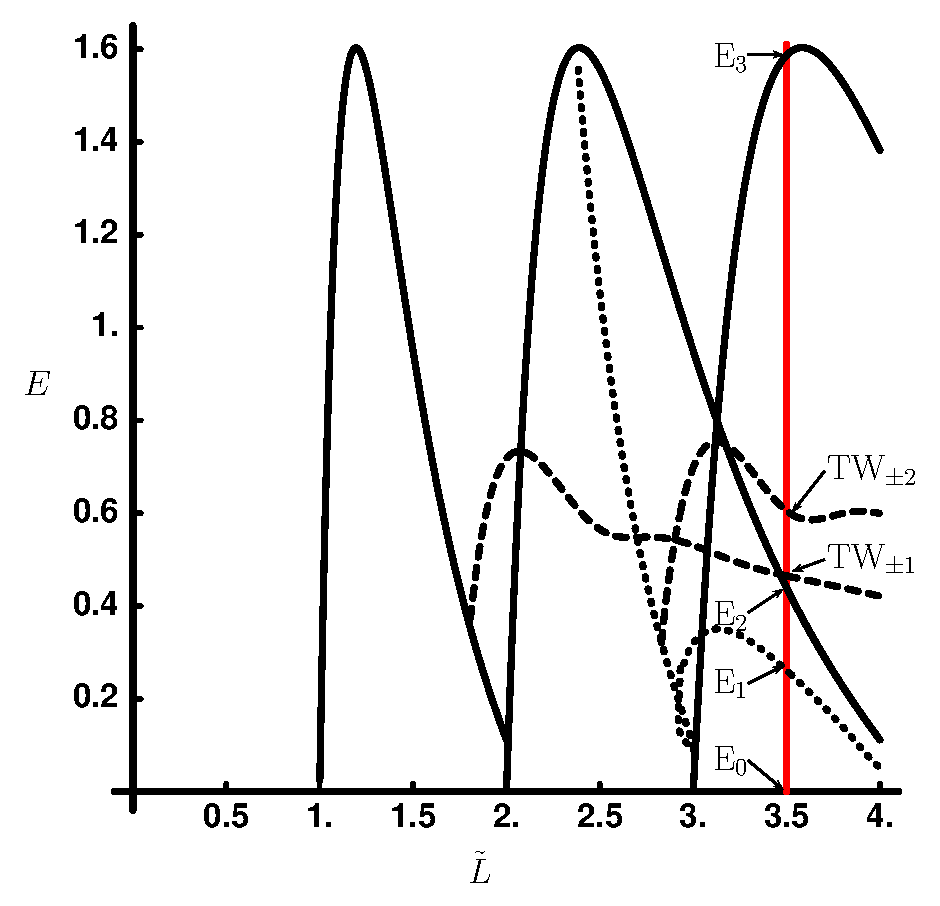
\includegraphics[width=0.5\textwidth]{figs_bmp/ksBifDiag_pst.eps}
\end{center}
\caption{
The energy \refeq{ksEnergy} of the \eqva\ and \reqva\ that
exist up to $L=22$, $\tildeL = 3.5014\ldots$, plotted as a function
of the system size $\tildeL = L/2\pi$ (additional \eqva, not present
at $L = 22$ are given in \refref{ksgreene88}). Solid curves denote
$n$-cell solutions \EQV{2} and \EQV{3}, dotted curves the GLMRT
\eqv\ \EQV{1},
and dashed curves the \reqva\ \REQV{\pm}{1} and \REQV{\pm}{2}.
The parameter $\alpha$ of \refrefs{KNSks90,ksgreene88} is
related to the system size by $\tildeL=\sqrt{\alpha/4}$.
        }
\end{figure}
%%%%%%%%%%%%%%%%%%%%%%%%%%%%%%%%%%%%%%%%%%%%%%%%%%%%%%%%%%%%%%%%%%

In the Fourier representation the \reqva\ time dependence is
\beq
 a_k(t) e^{-itc q_k} = a_k(0)
\,.
\ee{reqvaF}
Differentiating with respect to time, we obtain
the Fourier space version of the \reqv\ condition
\refeq{KSeqvCond},
\beq
 \pVeloc_k(a) - i q_k \velRel a_k = 0
\,,
\ee{reqvCondF}
which we solve for (time independent) $a_k$ and $c$.
Periods of spatially periodic {\eqva} are $L/n$ with integer $n$.
Every time the system size crosses  $\tildeL=n$,
$n$-cell states
are generated through pitchfork bifurcations off $u =0$
equilibrium.
Due to the translational invariance of {\KSe},
they form invariant circles
in the full \statesp.
In the $\bbU^+$ subspace considered here,
they correspond to $2n$ points, each shifted by $L/2n$.
For a sufficiently small $L$
the number of {\eqva} is small and
concentrated on the low wave-number end of the Fourier spectrum.

In a periodic box of size $L$
both \eqva\ and \reqva\ are  periodic solutions
embedded in 3-$d$ space, conveniently represented as loops in
$(u,u_x,u_{xx})$ space, see \reffig{f:KS22Equil}\,(\textit{d}).
In this representation the continuous translation symmetry
is automatic -- a rotation in the $[0,L]$ periodic domain only
moves the points along the loop. For an \eqv\ the points
are stationary in time; for \reqv\ they move in time, but in
either case, the loop remains invariant.
So we do not have the problem that we encounter in the Fourier
representation, where seen from the frame of one of the \eqva\
the rest trace out circles under the action of continuous symmetry
translations.

From \refeq{expan} we see that the origin $u(x,t) = 0$
has Fourier modes as the linear stability eigenvectors
(see \refappe{sec:stability}).  The $|k|<\tildeL$
long wavelength perturbations of the flat-front {\eqv}
are linearly unstable, while for
$|k|$ sufficiently larger than $\tildeL$ the short wavelength
perturbations are strongly contractive. The high $k$
eigenvalues, corresponding to rapid variations of the flame
front, decay so fast that the corresponding eigendirections
are physically irrelevant. Indeed, \refref{YaTaGiChRa08} shows that
the chaotic solutions of spatially extended dissipative
systems evolve within an inertial manifold spanned by a
finite number of physical modes, hyperbolically isolated from
a set of residual degrees of freedom with high $k$, themselves individually
isolated from each other.
The most unstable mode, nearest to $|k|=\tildeL/\sqrt{2}$,
sets the scale of the mean wavelength $\sqrt{2}$
of the KS `turbulent' dynamics,
see \reffig{f:ks_largeL}.


\subsection{\Rpo s, symmetries and \po s} \label{sec:KSePO}

The KS equation \refeq{ks} is time translationally invariant, and
space translationally invariant under the 1-$d$ Lie group of $O(2)$
rotations: if $u(x,t)$ is a solution, then $u(x+\shift,t)$ and
$-u(-x,t)$ are equivalent solutions for any $-L/2 < \shift \leq
L/2$.
As a result of invariance under $\Shift_{\shift/L}$,
KS equation can have \rpo\ solutions
with a profile $u_p(x)$, period $\period{p}$, and a
nonzero shift $\shift_p$
\beq
  \Shift_{\shift_p/L}u(x,\period{p}) =
  u(x+\shift_p,\period{p}) = u(x,0) = u_p(x)\,.
\label{KSrpos}
\eeq
{\Rpo s} \refeq{KSrpos} are periodic in
$\velRel_p=\shift_p/\period{p}$ co-rotating frame (see
\reffig{f:MeanVelocityFrame}), but in the stationary frame their
trajectories are quasiperiodic.  Due to the reflection symmetry
\refeq{KSparity} of KS equation, every {\rpo} $u_p(x)$ with shift
$\shift_p$ has a symmetric partner $-u_p(-x)$ with shift $-\shift_p$.

Due to invariance under reflections, KS equation can also have
\rpo s {\em with reflection}, which are
characterized by a profile $u_p(x)$ and
period $\period{p}$
\beq
  \Refl u(x+\shift,\period{p}) =
  -u(-x-\shift,\period{p}) = u(x+\shift,0) = u_p(x)
  \,,
\label{KSpos}
\eeq
giving the family of equivalent solutions
parameterized by $\shift$
(as the choice of the reflection point is arbitrary,
the shift can take any value in $-L/2 < \shift \leq L/2$).

Armbruster \etal\rf{AGHks89,AGHO288} and Brown and
Kevrekidis\rf{BrKevr96} (see also \refref{Krupa90}) link the
birth of \rpo s to an infinite period global bifurcation
involving a heteroclinic loop connecting equilibria or a
bifurcation of \reqva, and also report creation of \rpo\
branches through bifurcation of \po s.

As $\shift$ is continuous in the interval $[-L/2, L/2]$,
the likelihood of a \rpo\ with $\shift_p = 0$ shift is zero,
unless an exact periodicity is enforced by a discrete symmetry,
such as the dihedral symmetries discussed above.
If the shift $\shift_p$ of a \rpo\ with period $\period{p}$ is such
that $\shift_p /L$ is a rational number, then the orbit is
periodic with period $n\period{p}$.  The likelihood to find such \po s is
also zero.

However, due to the KS equation invariance under
the dihedral $D_n$ and cyclic $C_n$ subgroups, the following
types of \po s are possible:

{\bf (a)} The \po\ lies
within a subspace pointwise invariant under the action of
$D_n$ or $C_n$. For instance, for $D_1$ this is the
$\bbU^+$ antisymmetric subspace, $-u_p(-x) = u_p(x)$, and
$u(x,\period{p}) = u(x,0) = u_p(x)$. The periodic orbits
found in \refrefs{Christiansen97,lanCvit07} are
all in $\bbU^+$, as the dynamics is restricted to
antisymmetric subspace. For $L=22$ the dynamics in $\bbU^+$
is dominated by attracting (within the subspace)
heteroclinic connections and thus we have no periodic orbits
of this type, or in any other of the $D_n$--invariant
subspaces, see \refsect{sec:L22}.

{\bf (b)} The \po\ satisfies
\beq
	 u(x,t+\period{p})=\gamma u(x,t)\,,
	\label{eq:POspattemp}
\eeq
for some group element $\gamma\in O(2)$ such that
$\gamma^m=e$ for some integer $m$ so that the orbit repeats
after time $m \period{p}$ (see
\refref{golubitsky2002sp} for a general discussion of
conditions on the symmetry of a \po).
If an orbit is of reflection type \refeq{KSpos},
$\Refl\Shift_{\shift/L} u(x,\period{p}) =
-u(-x-\shift,\period{p}) = u(x,0)$, then it is pre-periodic
to a \po\ with period $2\period{p}$. Indeed, since
$(\Refl\Shift_{\shift/L})^2 = \Refl^2 = 1$, and the KS
solutions are time translation invariant, it follows from
\refeq{KSpos} that
\[
  u(x,2\period{p}) = \Refl\Shift_{\shift/L} u(x,\period{p}) =
  (\Refl\Shift_{\shift/L})^2 u(x,0) = u(x,0)\;.
\]
Thus any shift acquired during time $0$ to
$\period{p}$ is compensated by the opposite shift during
evolution from $\period{p}$ to $2 \period{p}$.
All periodic orbits we have found for $L=22$ are of type
\refeq{eq:POspattemp} with $\gamma=R$. Pre-periodic orbits
with $\gamma\in C_n$ have been found by Brown and
Kevrekidis\rf{BrKevr96} for KS system sizes larger than ours,
but we have not found any for $L=22$.
Pre-periodic orbits are a hallmark of any dynamical system
with a discrete symmetry, where they have a natural
interpretation as \po s in the fundamental
domain\rf{CvitaEckardt,DasBuch}.

\section{Energy transfer rates}
\label{sec:energy}

In physical settings where the observation times are much
longer than the dynamical `turnover' and Lyapunov times
(statistical mechanics, quantum physics, turbulence) periodic
orbit theory\rf{DasBuch} provides highly accurate predictions
of measurable long-time averages such as the dissipation and
the turbulent drag\rf{GHCW07}. Physical predictions have to
be independent of a particular choice of ODE representation
of the PDE under consideration and, most importantly,
invariant under all symmetries of the dynamics. In this
section we discuss a set of such physical observables for the
1-$d$ KS invariant under reflections and translations. They
offer a representation of dynamics in which the symmetries
are explicitly quotiented out. We shall use these
observables in \refsect{sec:energyL22} in order to
visualize a set of solutions on these coordinates.

The {space average} of a function $\obser = \obser(\pSpace,t) = \obser(u(x,t))$  on
the interval $L$,
\beq
    \expct{\obser} = \Lint{\pSpace}\, \obser(\pSpace,t)
    \,,
    \label{rpo:spac_ave}
\eeq
is in general time dependent.
Its mean value is given by the {time average}
\beq
\timeAver{\obser}
    =
\lim_{t\rightarrow \infty} \frac{1}{t} \int_0^t \! d\tau \, \expct{\obser}
    =
\lim_{t\rightarrow \infty} \frac{1}{t} \int_0^t \!
    \Lint{\tau}  d\pSpace\, \obser(\pSpace,\tau)
    \,.
\label{rpo:tim_ave}
\eeq
The mean value of $\obser = \obser(u_\stagn) \equiv \obser_\stagn$ evaluated on
\eqv\ or {\reqv} $u(\pSpace,t) = u_\stagn(\pSpace-ct)$, labeled by  $q$ as in 
\refeq{reqva}, is
\beq
\timeAver{\obser}_\stagn = \expct{\obser}_\stagn = \obser_\stagn\,.
\label{rpo:u-eqv} \eeq 
Evaluation of the infinite time average
\refeq{rpo:tim_ave} on a function of a \po\ or \rpo\
$u_p(\pSpace,t)=u_p(\pSpace+\shift_p,t+\period{p})$ requires only a single
$\period{p}$ traversal,
\beq
  \timeAver{\obser}_p = \frac{1}{\period{p}}
    \int_0^{\period{p}} \! d\tau \, \expct{\obser}
\,.
\label{rpo:u-cyc}
\eeq

Equation \refeq{ks} can be written as
\beq
    u_t=- V_x
        \,,\qquad
    V(x,t)={\textstyle\frac{1}{2}}u^2+u_{x} + u_{xxx}
    \,.
\ee{ksPotent}
If $u$ is `flame-front velocity' then \expctE, defined in
\refeq{eq:stdks}, can be interpreted as the mean energy
density. So, even though KS is a phenomenological
small-amplitude equation, the time-dependent $L^2$ norm
of $u$,
\beq
    \expctE=
  \Lint{\pSpace}
  V(x,t)=
  \Lint{\pSpace} \frac{u^2}{2}
  \,,
  \label{ksEnergy}
\eeq
has a physical interpretation\rf{ksgreene88} as the average `energy'
density of the flame front. This analogy to the mean kinetic energy
density for the Navier-Stokes motivates what follows.

The energy \refeq{ksEnergy} is intrinsic to the flow,
independent of the particular ODE basis set chosen to
represent the PDE. However, as the Fourier amplitudes are
eigenvectors of the translation operator, in the Fourier
space the energy is a diagonalized quadratic norm,
\beq
\expctE
          =  \sum_{k=-\infty}^{\infty} E_k
\,,\qquad
E_k =
    {\textstyle\frac{1}{2}}|a_k|^2
\,,
\ee{EFourier}
and explicitly invariant term by term
under translations
\refeq{eq:shiftFour}
and reflections \refeq{KSparity}.

Take time derivative of the energy density \refeq{ksEnergy},
substitute \refeq{ks} and integrate by parts. Total derivatives vanish
by the spatial periodicity on the $L$ domain:
\bea
   \dot{\expctE} &=&
     \expct{u_t \, u}
         = - \expct{\left({u^2}/{2} + u_{x} + u_{xxx}\right)_x u }
    \continue
    &=&
\expct{ u_x \, {u^2}/{2} + u_{x}^2 + u_x \, u_{xxx}}
    \,.
\label{rpo:ksErate}
\eea
The first term in \refeq{rpo:ksErate} vanishes by
integration by parts,
\(
3 \expct{ u_x \, u^2}= \expct{(u^3)_x} = 0
\,,
\)
and integrating the third term by parts yet again
one gets\rf{ksgreene88} that the energy variation
\beq
   \dot{\expctE} = P - D
                \,,\qquad
      P =  \expct{u_{x}^2}
                \,,\quad
      D =  \expct{u_{xx}^2}
\ee{EnRate}
balances the power $P$ pumped in by anti-diffusion $u_{xx}$
against the energy dissipation rate $D$
by hyper-viscosity $u_{xxxx}$
in the KS equation \refeq{ks}.

The time averaged energy density  $\timeAver{E}$
computed on a typical orbit goes to a constant, so
the mean values \refeq{rpo:tim_ave} of drive and dissipation
exactly balance each other:
\beq
    \timeAver{\dot{E}}  =
    \lim_{t\rightarrow \infty}
        \frac{1}{t} \int_0^t d\tau \, \dot{\expctE}
=
      \timeAver{P} - \timeAver{D}
= 0
    \,.
\ee{rpo:EtimAve}
In particular, the \eqva\
and \reqva\ fall onto the diagonal in \reffig{f:drivedrag}\,(\textit{a}),
and so do time averages computed on \po s and \rpo s:
\beq
\timeAver{E}_p =
\frac{1}{\period{p}} \int_0^\period{p}d\tau \, E(\tau)
    \,,\qquad
\timeAver{P}_p =
\frac{1}{\period{p}} \int_0^\period{p} d\tau \, P(\tau)
    =
      \timeAver{D}_p
    \,.
\label{poE}
\eeq
In the Fourier basis \refeq{EFourier} the conservation of energy on average
takes form
\beq
0 = \sum_{k=-\infty}^{\infty} ( q_k^2 - q_k^4 )\,
    \timeAver{E}_k
\,,\qquad
E_k(t) =  {\textstyle\frac{1}{2}} |a_k(t)|^2
\,.
\ee{EFourier1}
The large $k$ convergence of this series is insensitive to the
system size $L$; $\timeAver{E_k}$ have to decrease much faster than
$q_k^{-4}$.
Deviation of $E_k$ from this bound for small $k$ determines the active modes.
For \eqva\ an $L$-independent bound
    on $E$ is given by Michelson\rf{Mks86}.
The best current bound\rf{GiacoOtto05,bronski2005} on the long-time limit
of $E$
as a function of the system size $L$ scales as
$E \propto L^2$.
